\begin{figure}
\begin{center}
    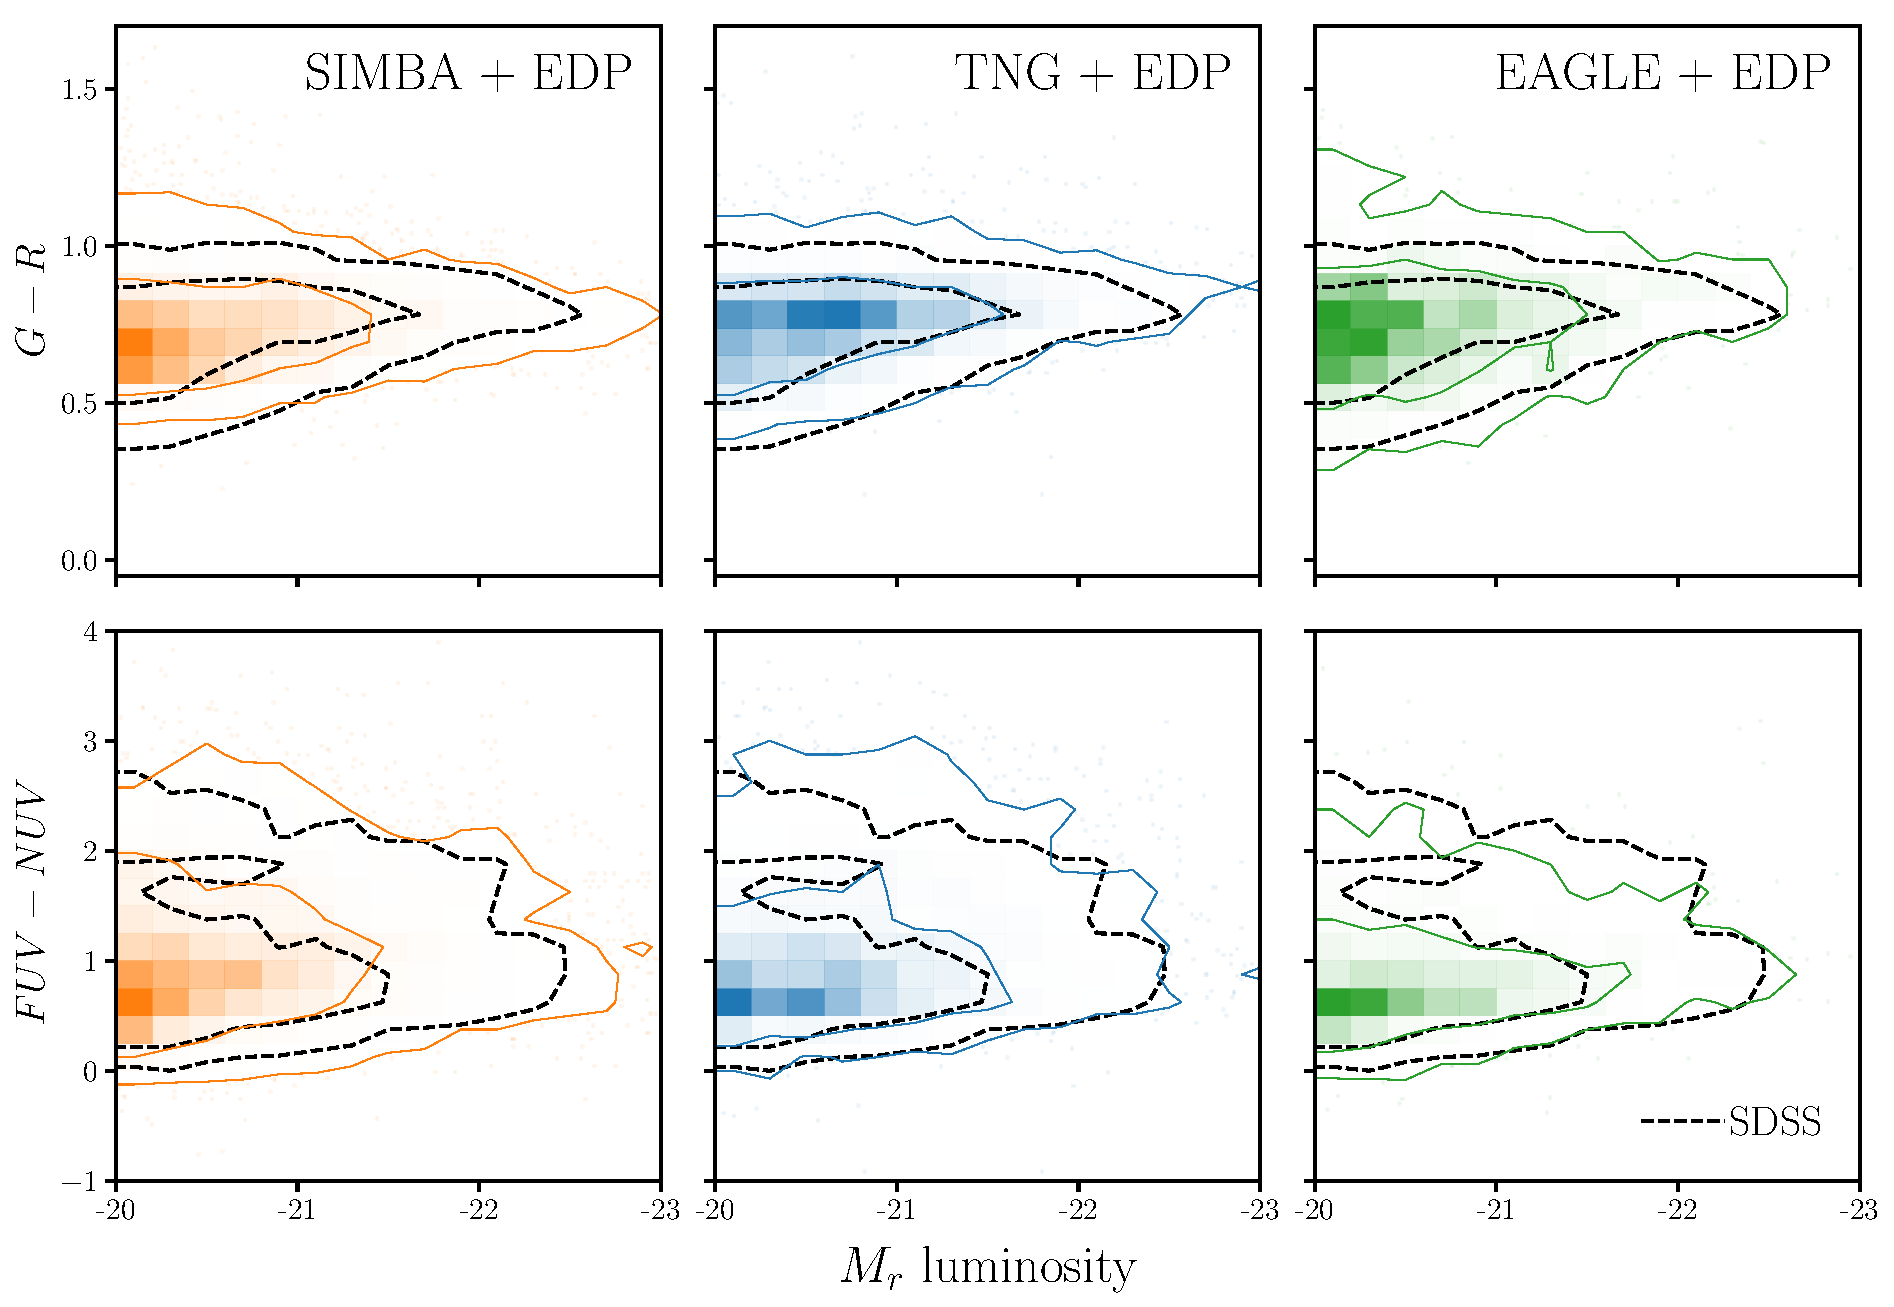
\includegraphics[width=0.9\textwidth]{figs/abc_observables.pdf}
    \caption{\label{fig:dem}
    The optical, $(\gr) - M_r$ (top), and UV, $(\fnuv) - M_r$ (bottom),
    color-magnitude relations predicted by our \eda~prescription
    for the SIMBA (orange), TNG (blue), and EAGLE (green) hydrodynamical
    simulations. For the \eda~parameters of each simulation, we use the
    median of the posterior distributions inferred using ABC. For
    comparison, we include the color-magnitude relations of SDSS (black
    dashed). Comparing the color-magnitude relations above to those without
    dust attenuation in Figure~\ref{fig:obs}, we see that dust
    \emph{dramatically} impacts the color-magnitude relations. 
    Dust attenuation must be accounted for when interpreting and comparing
    simulations. Furthermore, with our \eda~prescription, all three
    simulations reproduce the color-magnitude relations of SDSS
    observations.  \emph{Since the different simulations can reproduce
    observations just by varying dust, dust significantly limits our ability to
    constrain the underlying physical processes of galaxy formation
    models.}
    }
\end{center}
\end{figure}

\section{Results} \label{sec:results}
% dust model can reproduce color magnitude relation
Without dust attenuation, all of the hydrodynamical simulations struggle to 
reproduce the $(\gr) - M_r$ and $(\fnuv) - M_r$ relations of SDSS (Figure~\ref{fig:obs}). 
\chedit{ 
    Both in the optical and UV, the simulations predict galaxies with significantly bluer
    colors than SDSS galaxies.
    The simulations also predict optically blue luminous galaxies with $M_r <
    -21.5$ that are not found in the observations; this is particularly
    noticeable for SIMBA and TNG. 
    Simulated galaxies in SIMBA also have a significantly broader distribution
    of $\gr$ colors than SDSS galaxies.
    Meanwhile, all of the simulations predict a broader distribution of $\fnuv$  
    color than SDSS.
    In fact, SIMBA and TNG predict a significant number of luminous galaxies,
    $M_r < -22$, with $\fnuv > 2$ colors, which extends beyond SDSS observations.
}

\emph{With our \eda~prescription, all three simulations produce
color-magnitude relations much more consistent with SDSS observations.}
In Figure~\ref{fig:dem}, we present the optical and UV color-magnitude
relations predicted by the 
\eda~for the SIMBA (orange), TNG (blue), and EAGLE (green) simulations. 
For the \eda~parameters, we use the median of the inferred posterior distributions (Figure~\ref{fig:abc}). 
We include the color-magnitude
relations of SDSS observations (black-dashed) comparison. The contours mark 
the $68$ and $95$ percentiles of the distributions. 

Dust dramatically impacts the observables of simulations. 
The \eda~affects the optical and UV color-magnitude relations in three
major ways to produce good agreement with SDSS. 
\chedit{
    First, the \eda~significantly reddens the simulated galaxies in the optical: 
    $\gr$ colors are ${\gtrsim}0.25~mag$ redder than the optical
    color-magnitude relation in Figure~\ref{fig:obs} and match the $\gr$
    distribution of SDSS. 
    Second, the \eda~significantly reddens non-quiescent ($\log\ssfr > -11$)
    galaxies in the UV.  
    While quiescent galaxies have intrinsically red UV colors, $\fnuv > 0.5$,
    that generally agree with SDSS, the rest of the galaxies are intrinsically
    bluer in the UV than observations. 
    The \eda~reddens their $\fnuv$ colors by ${\gtrsim}0.5~mag$.
    Lastly, the \eda~also attenuates non-quiescent galaxies.
    As a result, there are no longer luminous galaxies that are blue in the
    optical or UV --- consistent with observations.
}

\begin{figure}
\begin{center}
    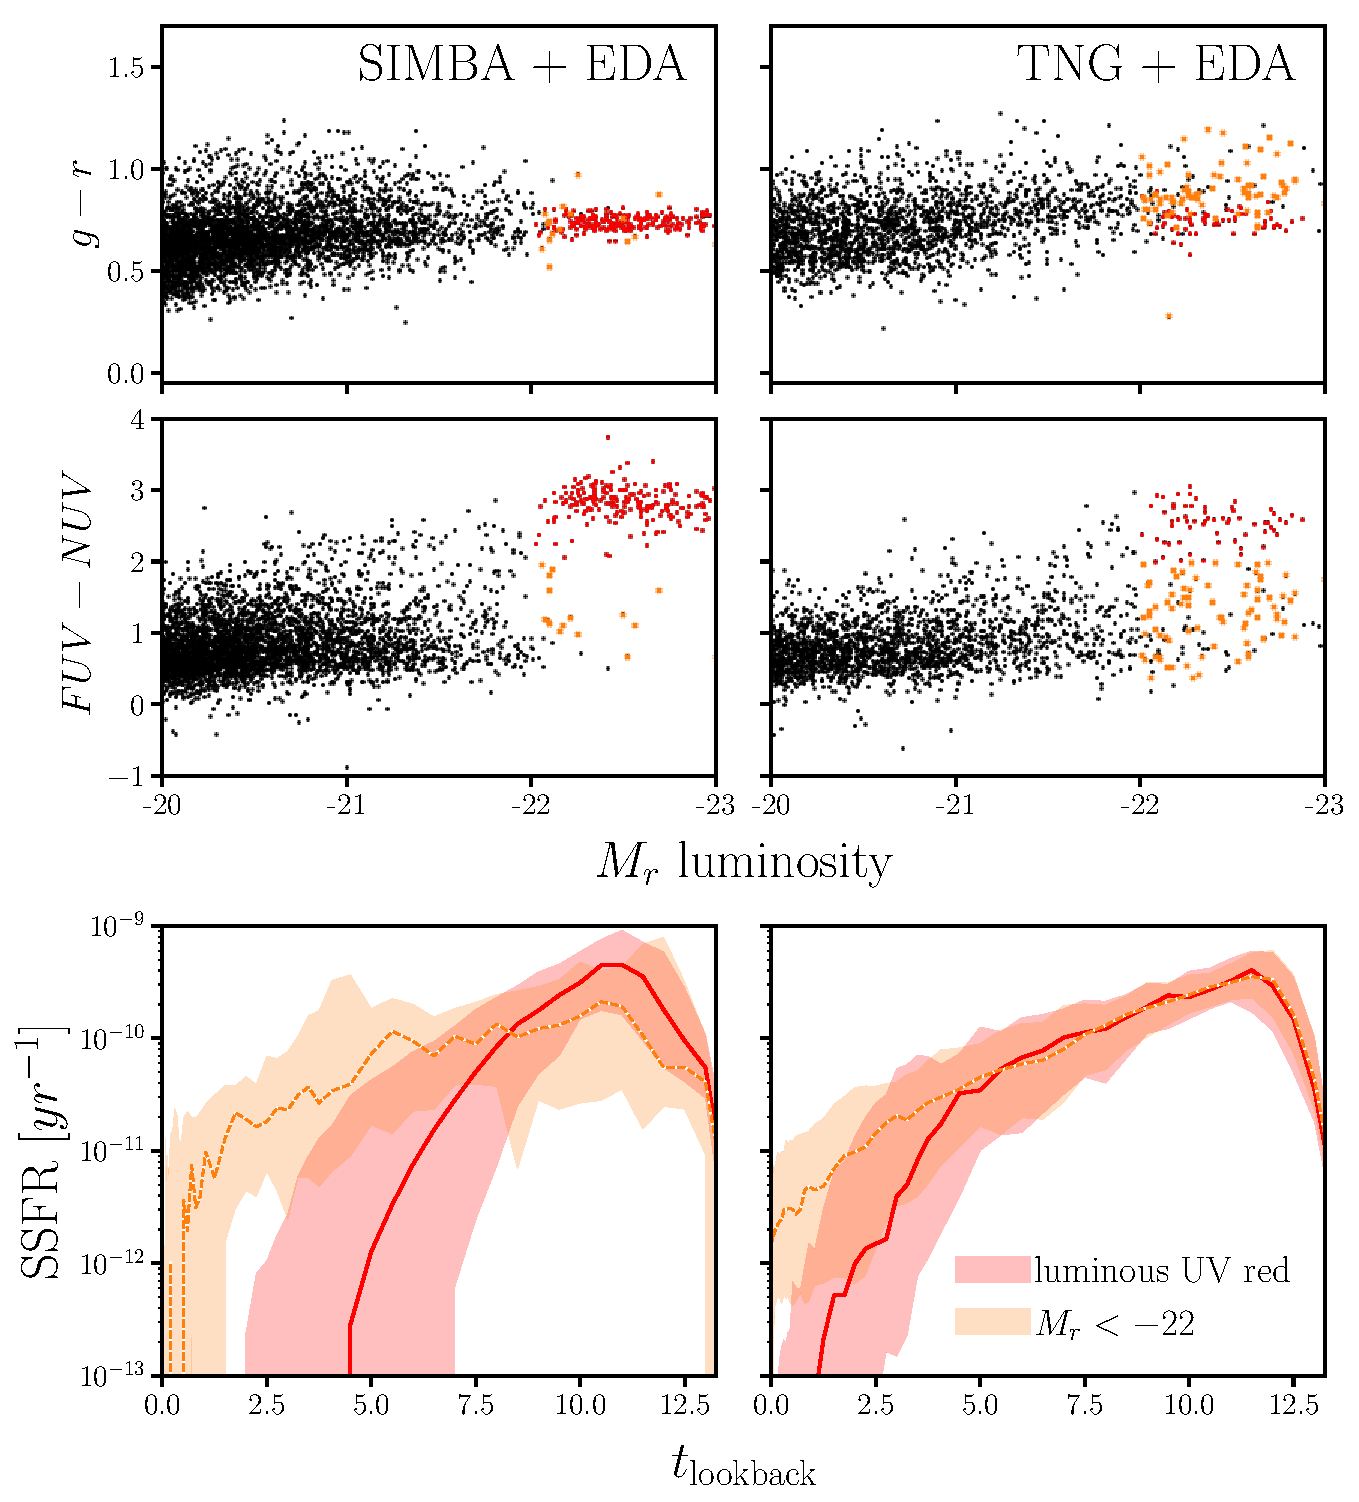
\includegraphics[width=0.6\textwidth]{figs/abc_observables_uvred.pdf}
    \caption{\label{fig:uv_sfh}
    \chedit{
        The SFHs of luminous UV red galaxies (red) in SIMBA (left) and TNG
        (right) that cause the discrepancy between the color-magnitude
        relations predicted by the \eda~and SDSS observations. 
        We include the SFHs of quiescent galaxies with matching luminosities, 
        $M_r < -22$, for comparison (orange). 
        The top and center panels mark the luminous UV red and the other $M_r < -22$
        galaxies in the \eda~predicted optical and UV color-magnitude relations,
        respectively. 
        In the bottom panels, we present the median SSFH of these galaxies 
        with the shaded regions representing the 68 percentiles of the SSFH. 
        In both TNG and SIMBA, the luminous UV red galaxies have negligible
        star formation within the last 2 Gyrs, unlike the other quiescent
        galaxies, \tks{suggesting these may be too strongly quenched compared to the SDSS sample.}
        %\emph{Therefore, SIMBA and TNG predict luminous UV red galaxies not
        %found in observations because their prescription for star formation
        %quenching is too efficient in the most massive galaxies.}
    }
    }
\end{center}
\end{figure}

\chedit{
    Despite the substantial improvement in the color-magnitude relation
    agreement with the \eda, there is still one significant discrepancy: the
    presence of luminous UV red galaxies with $M_r > -22$ and $\fnuv > 2$
    that are not found in observations. 
    This galaxy population, which consists of quiescent galaxies with
    $\sfr\lesssim 10^{-2}M_\odot/yr$, is especially pronounced in the UV
    color-magnitude of SIMBA but also present in TNG. 
    They are also present in the UV color-magnitude predictions without dust
    attenuation~(Figure~\ref{fig:obs}). 
    Since these galaxies are luminous and they have intrinsic $\fnuv > 2$, 
    dust attenuation cannot remove them from the UV color-magnitude relation.
    In other words, the excess luminous UV red galaxies predicted by SIMBA and
    TNG are irreconcilable even with dust attenuation \tks{in the flexible \eda framework (based on comment by Daniel, I added the note that the EDA is flexible)}. 
}

\chedit{ 
    In order to understand the origin of the luminous UV red galaxies in SIMBA
    (left) and TNG (right), we examine their star formation histories in
    Figure~\ref{fig:uv_sfh}.
    The top and center panels mark the luminous UV red galaxies on the optical
    and UV color-magnitude relations predicted by the \eda~(red). 
    The bottom panels present the median specific SFH (SSFH), $\ssfr$ as a
    function of lookback time, $t_{\rm lookback}$, with the shaded regions
    representing the 68 percentile of the SSFH.
    For comparison, we include the SSFHs of other quiescent galaxies with 
    matching luminosities, $M_r < -22$ (orange).
    The SSFHs reveal that, unlike other quiescent galaxies, the luminous UV red
    galaxies of SIMBA and TNG have almost no star formation within the last
    $t_{\rm lookback} \lesssim 2$ Gyr.
    With no recent star formation contributing to the SED in $FUV$ wavelength,
    these galaxies have faint $FUV$ magnitudes and, thus, high $\fnuv$ color.  
    The luminous UV red galaxies in SIMBA and TNG, which are not found in
    observations, \tks{could be} a consequence of star formation quenching being too
    efficient in the most massive quiescent galaxies.
}

\chedit{
    The SSFHs in Figure~\ref{fig:uv_sfh} also reveal that luminous UV red
    galaxies in SIMBA have a substantially different SSFH than other quiescent
    galaxies. 
    Besides the lack of recent star formation, the luminous UV red
    galaxies peak their star formation earlier than other quiescent galaxies at
    $t_{\rm lookback}\sim 11$ Gyr and have a more rapid decline in star
    formation. 
    In contrast, the luminous UV red galaxies in TNG have overall similar
    SSFHs. 
    This difference in SFH suggests that a distinct star formation quenching
    mechanism is responsible for the luminous red galaxies in SIMBA. 
    In another paper of the IQ series (Choi et al. in prep), we examine this
    SFH difference in further detail and present its impact on the quiescent 
    fraction evolution over $0 < z < 3$. 
}

% SIMBA discrepancy
%\chedit{
%    For SIMBA, although the \eda~prescription significantly improves the
%    agreement, it still struggles to reproduce the SDSS color-magnitude relations. 
%    The overall agreement is significantly worse than TNG and EAGLE: the median
%    ABC distance metric (Eq.~\ref{eq:distance}) of the posterior 
%}
%\todo{UPDATE NUMBERS: 
%    $\rho = 3.7\times10^{-3}, 3.2\times10^{-3}$ for TNG and EAGLE while 
%    $\rho = 6.6\times10^{-3}$ for SIMBA. 
%}
%\todo{UPDATE: 
%    Moreover, SIMBA+\eda~preoduces a optically bluer red sequence and a much
%    broader UV color-magnitude relation. 
%}
%The inferred \eda~parameters for SIMBA also differ significantly from the
%parameters of TNG and EAGLE (Figure~\ref{fig:abc}). 
%\chedit{
%    We infer the opposite $\ssfr$ dependence for the amplitude and slope of
%    dust attenuation than TNG or EAGLE.
%    These discrepancies are primarily driven by the excess of two galaxy
%    subpopulations in SIMBA. 
%    First, are quiescent galaxies with $\sfr=0$ at $z=0$ and SFHs that peak at
%    $z\sim2$ and fully quenched at $z\sim1$.
%    Unlike other quiescent galaxies in SIMBA, they have had no star formation
%    in the past $\gtrsim 2{\rm Gyr}$.  
%    These galaxies have highly red intrinsic (without dust) UV color:
%    $\fnuv > 2.5{\rm mag}$.
%    While, TNG and EAGLE also have galaxies with $\fnuv > 2.5{\rm mag}$, they
%    do not have high luminosity $M_r > -22$ (Figure~\ref{fig:obs}). 
%    Furthermore, unlike the UV red galaxies in SIMBA, they do not have fully 
%    quenched SFHs with no recent star formation; instead, they have SFHs that
%    are similar to other quiescent galaxies. 
%    The other population that drives the SIMBA discrepancy is the high
%    $\ssfr > 10^{-9.5}yr^{-1}$ ``starburst'' galaxies with
%    $M_*<10^{10}M_\odot$, which lie significantly above the SFS and are {\em
%    only} present in SIMBA (Figure~\ref{fig:smf_msfr}). 
%    This starburst population, which has also been identified in
%    \cite{dave2019} (see their Figures~5 and 6) is caused by excess gas in
%    low-mass galaxies at $z=0$. 
%}

%\chedit{
%    Without dust attenuation, both SIMBA populations strongly disagree with the
%    SDSS color-magnitude relation (Figure~\ref{fig:obs}). 
%    The UV red SIMBA galaxies have $\fnuv > 2.5$ over the entire luminosity
%    range.  
%    This is significantly redder than SDSS, which has only few galaxies with 
%    $\fnuv > 2.5$ and none that are luminous, $M_r > -21.5$.
%    Meanwhile the low mass starbursts have blue $\gr < 0.25$ and 
%    $-20 < M_r < -21$. 
%    This is significantly bluer than the SDSS $\gr \gtrsim 0.4$ limit and also
%    bluer than the SF galaxies in TNG and EAGLE. 
%    In order to reconcile these differences between SIMBA and SDSS, the
%    \eda~prescription imposes a steep attenuation curve with significant UV
%    attenutaion on the UV red galaxies so that they are excluded by our $M_{\rm
%    FUV}, M_{\rm NUV} < -10$ completeness limit. 
%    On the other hand, the \eda~prescription imposes a shallower attenuation
%    curve with high $A_V$ for the low mass starburst galaxies so that they are
%    excluded by our $M_r < -20$ completeness limit.
%    Despite removing the excess $\fnuv > 2.5$  and $\gr < 0.25$ galaxies, our
%    \eda~prescription, with its linear dependence on $\log M_*$ and $\log\ssfr$
%    struggles to accurately reproduce the SDSS color-magnitude relations. 
%    If we exclude the UV red and $\ssfr > 10^{-9.5}{yr}^{-1}$ starburst galaxies 
%    and run the \eda~for SIMBA using median values of the TNG or EAGLE posteriors 
%    for the \eda~parameters, we find similar level of agreement with SDSS as TNG 
%    and EAGLE. 
%}

% comparison to literature 
Previous works in the literature have also compared simulations with different
dust prescriptions to observations in color-magnitude space. For EAGLE, 
\cite{trayford2015} calculate colors and luminosities with the {\sc Galaxev}
population synthesis models and a two-component screen model for dust. More
recently, \cite{trayford2017} calculated optical colors for EAGLE using {\sc
Skirt}, a Monte Carlo radiative transfer code~\citep{camps2015}, to model the
dust. At stellar masses and luminosities comparable to our SDSS sample, both 
\cite{trayford2015} and \cite{trayford2017} produce red sequences bluer than 
in GAMA observations. Also, \cite{trayford2015} predict an excess of luminous 
blue galaxies. Although a detailed comparison is difficult since both works 
compare to different observations, we note that with the \eda, EAGLE is able 
to successfully reproduce the position of the SDSS red sequence and does not 
predict a significant excess of luminous blue galaxies. Also using EAGLE and 
{\sc Skirt}, \cite{baes2019} find that they overestimtate the observed cosmic 
SED (CSED) in the UV regime and produce significantly higher $\fnuv$ color 
than GAMA. The \eda~for EAGLE predicts $\fnuv$ in good agreement with SDSS. 
%\cite{baes2019}: EAGLE+SKIRT SED compparison with GAMA Far UV is not attenuated enough. underrestimates optical and NIR
For TNG, \cite{nelson2018} calculate optical colors using a dust model that
includes attenuation due to dense gas birth clouds surrounding young stellar
populations and also due to simulated distribution of neutral gas and metals.
They find bluer red sequence peaks and a narrower blue cloud compared to SDSS.
We find neither of these discrepancies for the TNG+\eda. The \eda~provides a
simpler empirical framework for applying dust attenuation than the dust models
in these works. Yet, with its flexibility \tks{and low computation costs,} we are able to \tks{fully
explore our dust parameters and find the best-fit attenuation, producing}
%produce 
optical and
UV color-magnitude relations that are in good agreement with observations.
%Furthermore, with its low computation costs we were able to fully
%explore our dust parameters. 
%better agreement than observations than these works.

% without being fit, the EDA reproduces the attenuation-slope relation and SF
% attenuation of SDSS observations  
\begin{figure}
\begin{center}
    %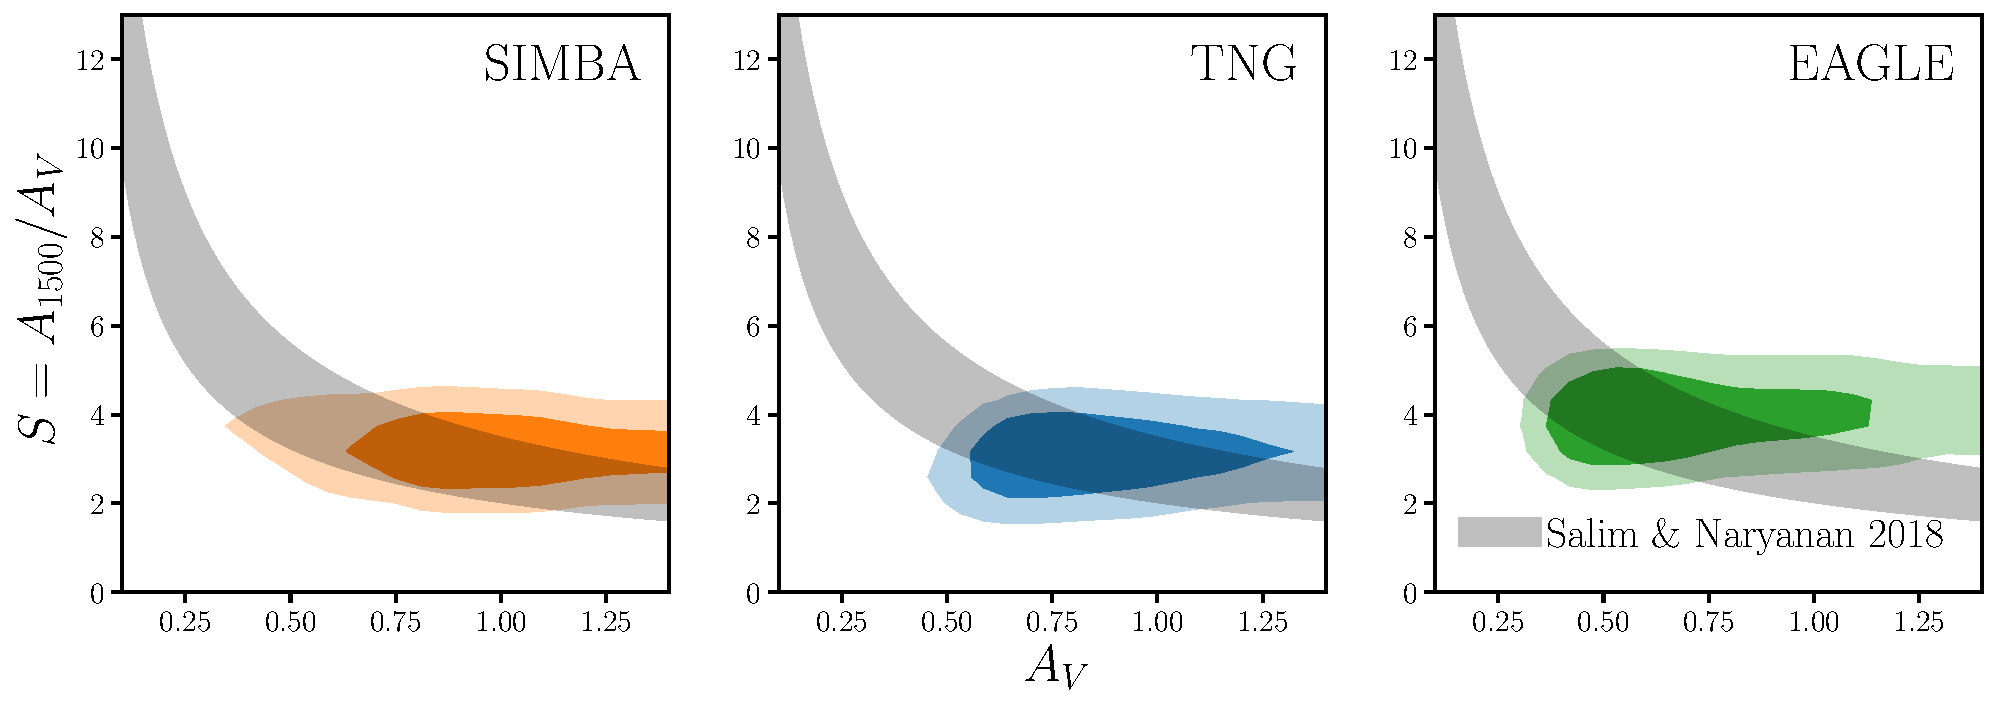
\includegraphics[width=0.9\textwidth]{figs/abc_slope_AV_starforming.pdf}
    \caption{\label{fig:slope}
    The attenuation-slope relation of star-forming galaxies ($\ssfr >
    10^{-11}yr^{-1}$), using the attenuation curves predicted by our  
    \eda~prescription for the median posterior parameter values of SIMBA
    (left), TNG (center) and EAGLE (right). 
    For comparison, we include the observed attenuation-slope relation
    from GSWLC2~\citep{salim2020}. 
    We use $A_V$ and $S = A(1500\AA)/A_V$ as measurements of attenuation and
    slope, respectively. 
    \chedit{
        \emph{The \eda~does not predict $A_V < 0.3$ because star-forming galaxies in
        the simulations are too lumnious and require significant attenuation to
        reproduce observations.}
        Beyond $A_V > 0.3$, however, there is good agreement between the
        attenuation-slope relation predicted by the \eda~and observations. 
    }
    }
\end{center}
\end{figure}

\subsection{Comparison to Dust Observations} \label{sec:reproduce}
With our \eda~prescription, we are able to accurately reproduce the
observed optical and UV color-magnitude relations with our simulations. 
In addition to  reproducing observations, since the \eda~assigns dust
attenuation curves to each simulated galaxy, we can compare the
\eda~attenuation curves to dust attenuation measured from
observations. 
We begin with the well-established attenuation-slope relation: star-forming
galaxies with higher dust attenuation have shallower attenuation curves. 
This relation is a consequence of dust scattering dominating absorption at
low attenuation while dust absorption dominates at high
attenuation~\citep{gordon1994, witt2000, draine2003, chevallard2013}. 
In Figure~\ref{fig:slope}, we present the attenuation-slope relation of
star-forming galaxies with $\ssfr > 10^{-11}yr^{-1}$ based on the
dust attenuation curves predicted by the \eda~for the median posteriors of
SIMBA (left), TNG (center) and EAGLE (right).
For comparison, we include the observed attenuation-slope relations of
GSWLC2 galaxies~\citep[grey shaded;][]{salim2020}.
For attenuation we use $A_V$ and for slope we use the UV-optical slope, $S
= A(1500\AA)/A_V$, commonly found in the literature. 
The contours mark the 68 and 95 percentiles. 
\chedit{
    Most noticably, we find that the \eda~does not predict $A_V < 0.3$. 
    This is not due to the selection function imposed by our forward model, but
    rather a consequence of SIMBA, TNG, and EAGLE predicting star-forming
    galaxies that are more luminous than observations.  
    All of the simulations have star-forming galaxies with intrinsic $M_r <
    -21$ and $\gr < 0.5$ (Figure~\ref{fig:obs}). 
    This is further corroborated by the $\sfr-M*$ relations in
    Figure~\ref{fig:smf_msfr}, where the simulations all have star-forming
    galaxies with $M_* > 10^{11}M_\odot$, not found in SDSS. 
    To reproduce the SDSS optical color-magnitude relation these galaxies would
    need to be significantly reddened and attenuated. 
    Hence, any dust prescription for the simulations would require high 
    $A_V$ for star-forming galaxies.
    Nevertheless, for $A_V > 0.3$, we find good agreement between the 
    attenuation-slope relation predicted by the \eda~and observations. 
}

%We note that the difference in the $A_V$ ranges is due to the $M_r$
%completeness limit imposed by our forward model (Section~\ref{sec:fm}).
%The GSWLC2 sample in \cite{salim2020} extends down to $M_* \sim
%10^{8.5}M_\odot$; however, the TNG and EAGLE samples do not extend below
%$M_* \sim10^{10}M_\odot$.
%\emph{The \eda~predicts attenuation-slope relations for TNG and EAGLE that
%are in excellent agreement with observations.} 

\begin{figure}
\begin{center}
    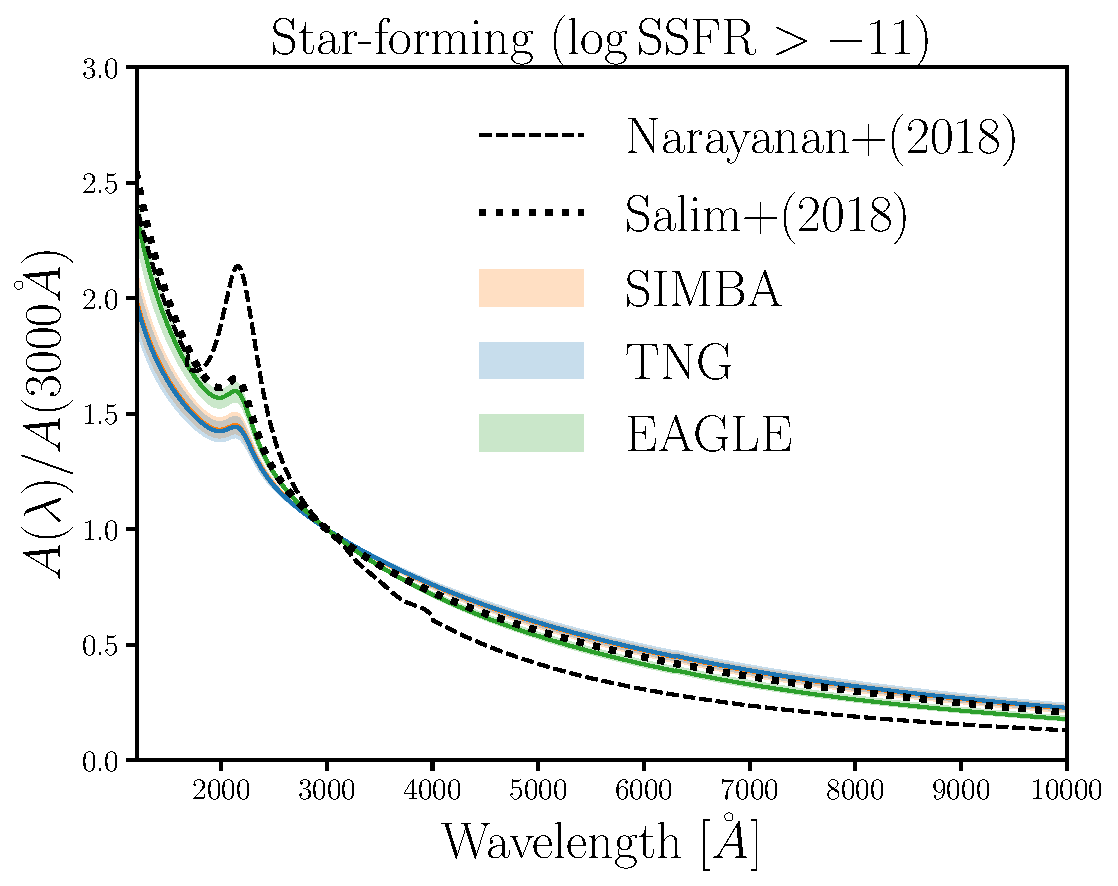
\includegraphics[width=0.5\textwidth]{figs/abc_sf_attenuation.pdf}
    \caption{\label{fig:sfatten}
    The normalized attenuation curves of star-forming galaxies predicted by
    the \eda~for median posterior parameter values of SIMBA (orange), TNG
    (blue), and EAGLE (green).  
    Galaxies with $\log \ssfr > -11~yr^{-1}$ are classified as star-forming. 
    The attenuation curves are normalized at $3000\AA$ and we mark the
    68 percentile of the attenuation curves with the shaded region.
    For comparison, we include $A(\lambda)/A(3000\AA)$ measurements from
    the~\cite{narayanan2018} radiative transfer simulation (dashed) and
    \cite{salim2018} observations (dotted).
    %The \cite{calzetti2000} and \cite{battisti2017} attenuation curves are shallower than the \eda~attenuation curves; however, they probe lower $M_*$ galaxies than our forward modeled TNG and EAGLE samples.  For attenuation curve from \cite{salim2018}, which probe a similar $M_*$ range, we find goood agreement. 
    {\em The \eda~predict attenuation curves of star-forming galaxies that
    are in good agreement with the attenuation curves measured from
    the simulation and observations in the literature.}
    %We also find good agreement with median attenuation curve of star-forming galaxies in the radiative transfer simulations of \cite{narayanan2018}.
    }
\end{center}
\end{figure}

In addition to the attenuation-slope relation, we can also directly compare
the attenuation curves predicted by the \eda~to measurements from
observations for star-forming galaxies. 
In Figure~\ref{fig:sfatten}, we present the normalized attenuation curves
of star-forming galaxies predicted by the \eda~for the median posterior
parameter values of SIMBA(orange), TNG (blue), and EAGLE (green).
We again define galaxies with $\ssfr > 10^{-11}{yr}^{-1}$ as star-forming.
The attenuation curves are normalized at $3000\AA$ and we present the
variation in the attenuation curves in the shaded region, 68 percentile. 
For comparison, we include $A(\lambda)/A(3000\AA)$ from the
\cite{narayanan2018} radiative transfer simulation (dashed) and 
observations~\citep[][dotted]{salim2018}. 
The attenuation curve from \cite{salim2018} corresponds to star-forming
galaxies with $M_* > 10^{10.5}M_\odot$, a similar $M_*$ range as our
forward modeled samples. 
Since we do not vary the UV bump in our \eda~prescription, we ignore any
discrepancies in the amplitudes of the bump. 
\emph{Overall, we find good agreement between the \eda~attenuation curves for
star-forming galaxies and the attenuation curves from observations and
simulations in the literature.}

%Again, the fact that we reproduce the detailed dust attenuation curves of star-forming galaxies in observations and simulations with the \eda~without fitting for them, highlights the advantages of a forward modeling approach. 

%The \eda~attenuation curves are slightly steeper than the \cite{calzetti2000} and \cite{battisti2017} curves. 
%These attenuation curves, however, are derived from $M_* < 10^{9.9}M_\odot$
%star-forming galaxies, which lie below the $M_*$ limit of our forward
%modeled TNG and EAGLE samples. 
%Meanwhile, the TNG and EAGLE \eda~attenuation curves are in good agreement
%with the \cite{salim2018} attenuation curve for $M_* > 10^{10.5}M_\odot$ star-forming galaxies. 
%They are also consistent with the median curve of \cite{narayanan2018}. 

%The \eda~attenuation curves are noticeably steeper than the \cite{calzetti2000} and \cite{battisti2017} curves.  These attenuation curves, however, are derived from $M_* < 10^{9.9}M_\odot$ star-forming galaxies --- below our $M_*$ range. 
%Since we find $\mdeltam < 0$ for both the TNG and EAGLE posteriors, the \eda~attenuation curves are consistent with \cite{calzetti2000} and \cite{battisti2017}. 


%\chedit{ 
%    The \eda~predicts higher dust attenuation at lower wavelenghts for
%    star-forming galaxies.
%    Without dust attenuation, both TNG and EAGLE predict star-forming galaxies
%    that are bluer in the optical and UV than observations
%    (Figure~\ref{fig:obs}).
%    To reproduce the SDSS, the \eda~significantly reddens star-forming galaxies.
%}
%In Figure~\ref{fig:raw_atten}, we also find that more massive star-forming
%galaxies have higher attenuation. This is because the simulations overpredict 
%luminous blue star-forming galaxies, which must be attenuated to reproduce
%observations. 


%At low attenuation, dust scattering dominates absoprtion so the 
%attenuation curve steepens because red light scatters isotropically while blue light
%scatters forward~\citep{gordon1994, witt2000, draine2003}. %, which causes more optical-to-IR light to escape the galaxy than UV light
%At high attenuation dust absorption is dominant and the attenuation curve is
%shallower~\citep{chevallard2013}. For the $A_V$ range probed by the DEM, the
%$A_V$--slope relation is in good agreement with GSWLC2 galaxies~\citep[black shaded][]{salim2020}.
%They are also consistent with \cite{leja2017}. We also compare our results to
%theoretical predictions from radiative transfer models, \cite{inoue2005}
%(dotted), the radiative transfer models considered in \cite{chevallard2013}
%(dot dashed), and \cite{trayford2020} (light shaded), which all predict shallower 
%attenuation curves than observations. This is also the case for the
%\cite{narayanan2018} attenuation curves (not included). 
%\emph{The attenuation curve slopes from the DEM for are in excellent
%agreement with observations and better reproduces the observed
%attenuation--slope relation than radiative transfer models.}
 

\begin{figure}
\begin{center}
    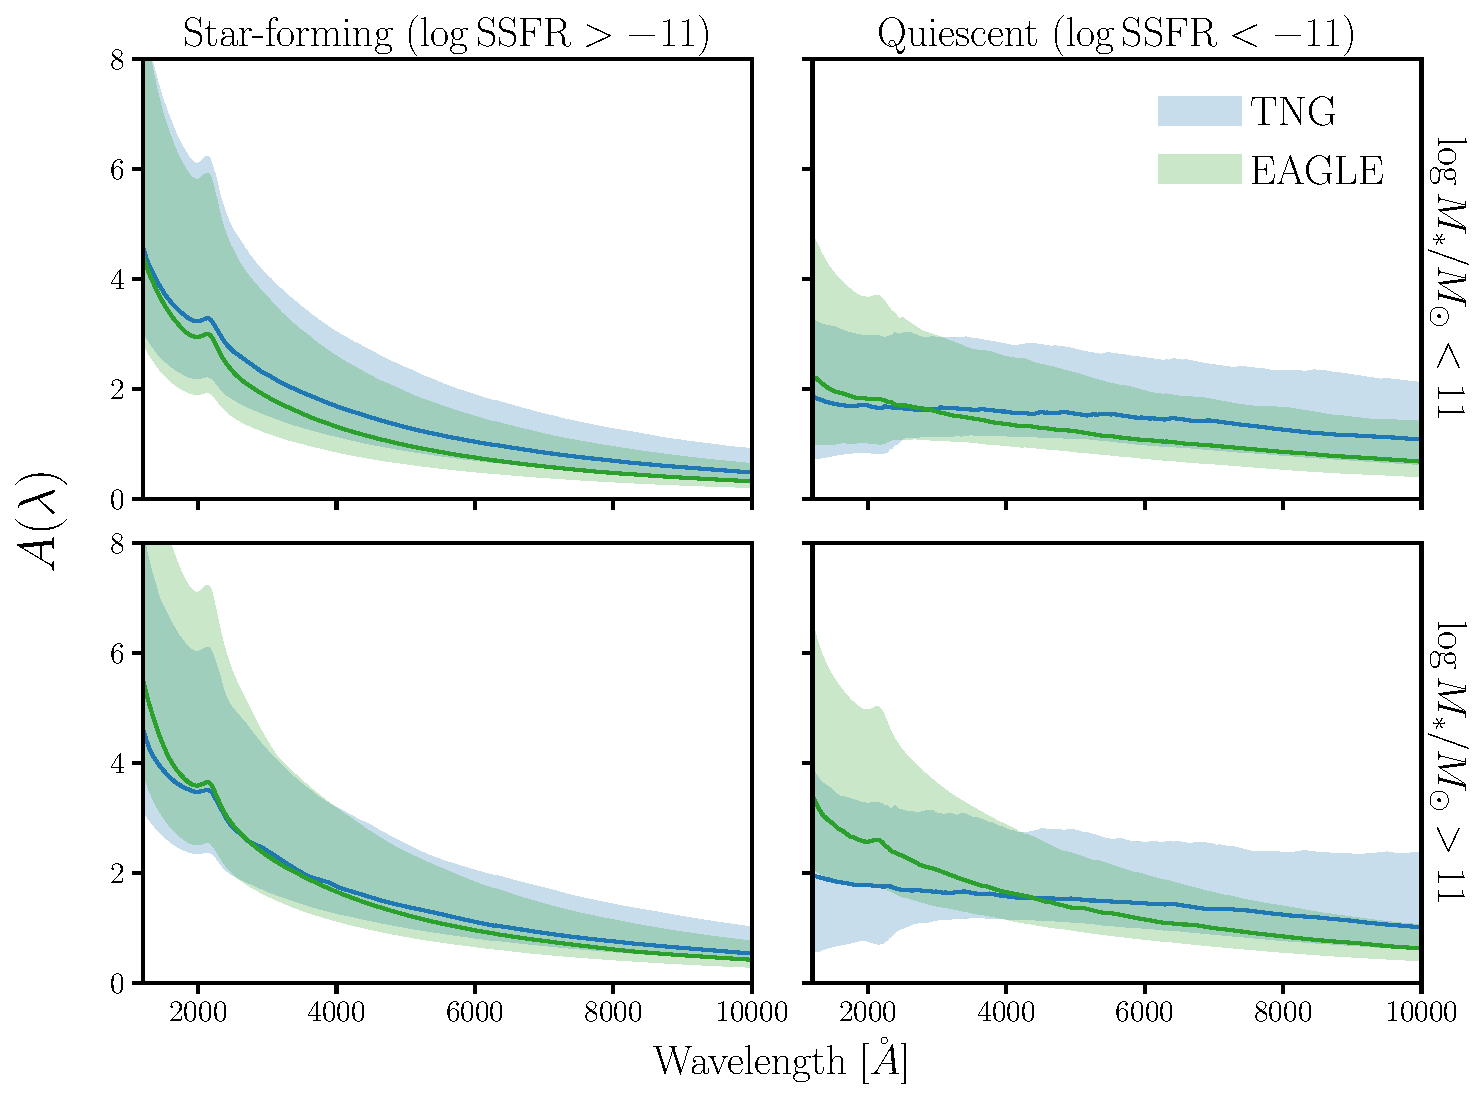
\includegraphics[width=0.85\textwidth]{figs/abc_attenuation_unormalized.pdf}
    \caption{\label{fig:raw_atten}
    Same as Figure~\ref{fig:atten} except the attenuation curves are not
    normalized at 3000$\AA$. Based on the \eda, quiescent galaxies have
    significant UV and optical dust attenuation. Furthermore, they have 
    significantly lower attenuation in the UV compared to star-forming 
    galaxies and have shallow attenuation curves overall.
    }
\end{center}
\end{figure}
\subsection{The Attenuation Curves of Quiescent Galaxies}  
We have demonstrated so far that the \eda~is able reproduce the observed UV and
optical color-magnitude relations and also predict dust attenuation curves
of star-forming galaxies consistent with observations and radiative transfer 
simulations. In addition, the \eda~also predicts dust attenuation curves of
quiescent galaxies. This is particularly valuable since there are many challenges 
to measuring attenuation curves for quiescent galaxies directly from observations. 
Methods that rely on IR luminosities can be contaminated by MIR emission from AGN
heating nearby dust~\cite{kirkpatrick2015}. Even SED fitting methods require 
accounting for AGN MIR emission~\citep{salim2016, leja2018, salim2018}. SED 
fitting methods also struggle to tightly constrain dust attenuation for quiescent 
galaxies since they are limited by the degeneracies with star formation history and 
metallicity.

With a forward modeling approach, we circumvent these challenges. We derive the 
attenuation curves necessary for quiescent galaxy population in simulations to
reproduce the observed optical and UV photometry.  In right panels of
Figure~\ref{fig:atten}, we present the attenuation curves of quiescent galaxies 
predicted by the \eda~model for the median posterior parameter values of TNG (blue) 
and EAGLE (green). In the top and bottom panels, we present galaxies with 
$M_* < 10^{11} M_\odot$ and $M_* > 10^{11} M_\odot$, respectively. 
We define galaxies with $\log {\rm SSFR} < -11$ as quiescent. The right panels 
of Figure~\ref{fig:raw_atten} are the same as in Figure~\ref{fig:atten}, except
the attenuation curves in Figure~\ref{fig:raw_atten} are not normalized. 

For both TNG and EAGLE posteriors, the \eda~predicts significant dust attenuation 
in quiescent galaxies. Compared to star-forming galaxies, however, they have 
lower attenuation in the UV and much shallower attenuation curves. The amplitude 
of the \eda~quiescent galaxy attenuation curves is driven by the fact that both
TNG and EAGLE --- without dust --- predict quiescent galaxies that are too 
luminous compared to observations. Hence, significant attenuation is necessary 
to lower their luminosity. Meanwhile, the shallow slope is driven by the
simulations predicting quiescent galaxies that are bluer in the optical but
redder in the UV than observations. The \eda~optically reddens the quiescent
galaxies but maintains a shallow enough slope to reproduce the UV
color-magnitude relation. This is also why TNG has a shallower slope than
EAGLE: TNG has an optically redder quiescent population and more quiescent
galaxies with high $\fnuv$ color. 

Given the challenges in observationally measuring attenuation curves of quiescent
galaxies, the predictions of the bestfit \eda~models for TNG and EAGLE
highlight the advantages of a forward modeling approach and provide valuable 
insights into dust attenuation in quiescent galaxies. \emph{Quiescent galaxies
have significant UV and optical attenuation with shallow attenuation curves.} 

 

\begin{figure}
\begin{center}
    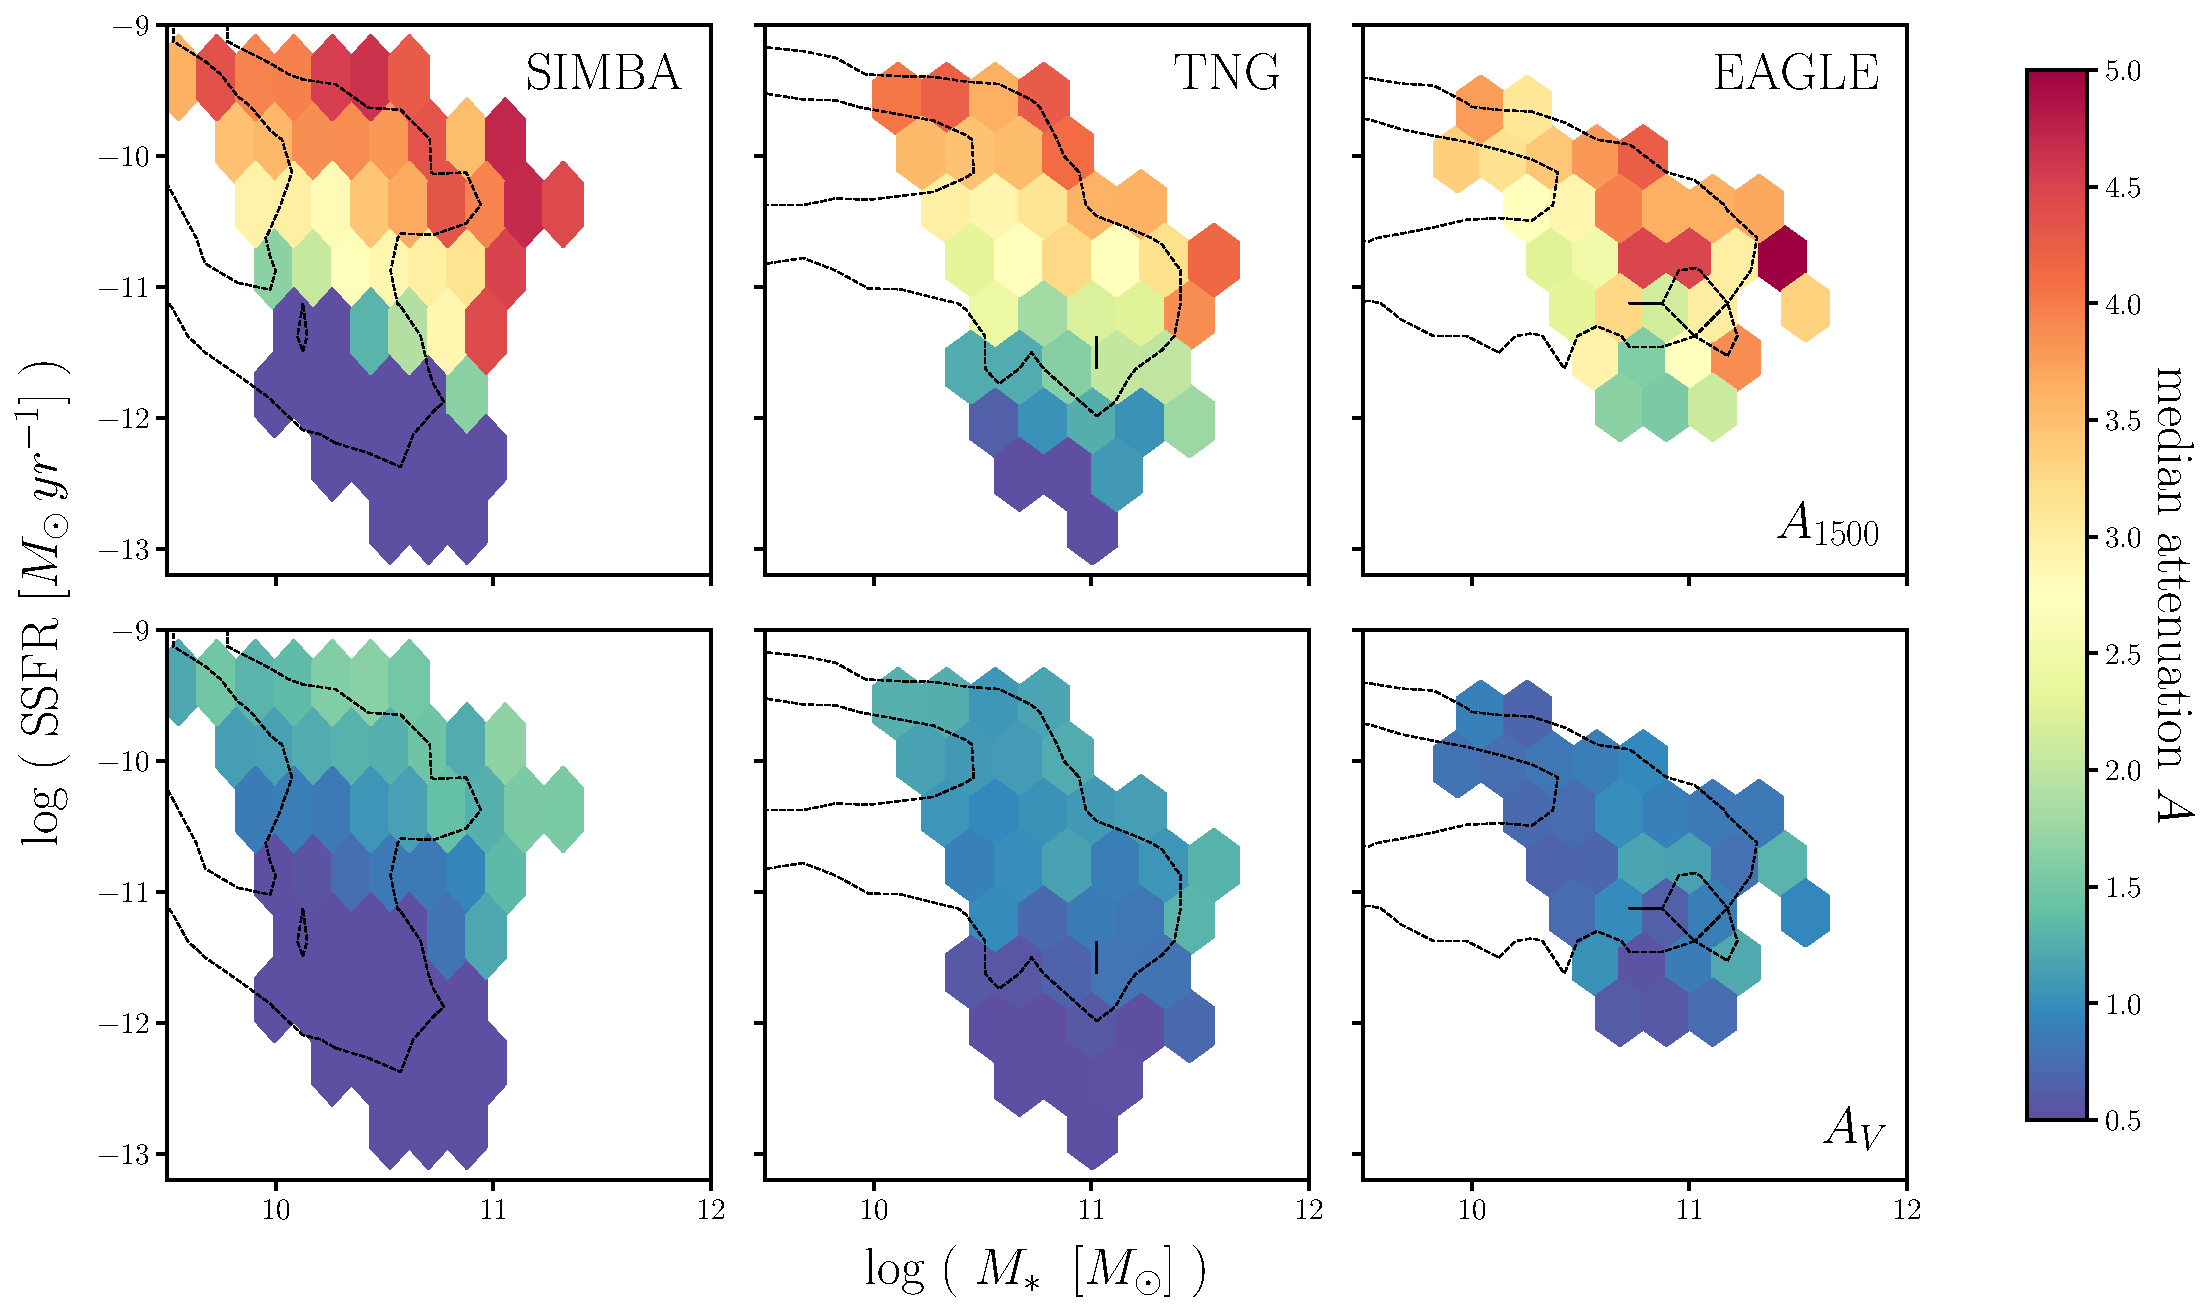
\includegraphics[width=0.9\textwidth]{figs/abc_av_mssfr.pdf}
    \caption{\label{fig:avmsfr}
        $M_*$ and $\ssfr$ dependence of dust attenuation at $1500 \AA$
        ($A_{1500}$; top) and at $5500\AA$ ($A_{V}$ bottom) predicted by the
        \eda~for SIMBA(left), TNG (center), and EAGLE (right). The colormap in each hexbin 
        represents the median attenuation for all simulated galaxies in the
        bin (right color bar). We only include bins with more than 10 galaxies.
        For reference, we include in each panel the $M_*-\ssfr$ relation of
        all galaxies from the simulations (black dashed).
        Overall, simulated galaxies with higher $M_*$ have higher dust
        attenuation at constant SSFR --- consistent with the literature.
        Furthermore, since previous works have primarily focused on star-forming
        galaxies, the \eda~provides new insight into the $\ssfr$ dependence of
        dust attenuation: simulated galaxies with higher $\ssfr$ have steeper
        attenuation curves. 
    }
\end{center}
\end{figure}

\subsection{The Galaxy -- Dust Connection}  
In the previous section, we presented the attenuation curves predicted by
the \eda~for quiescent galaxies. 
By comparing them to the attenuation curves of star-forming galaxies, we
found significant $\ssfr$ dependence in dust attenuation: quiescent galaxies
have attenuation curves with shallower slopes and lower amplitude than
star-forming galaxies. 
With the $M_*$ and $\ssfr$ dependent parameterization of our
\eda~prescription (Eqs~\ref{eq:tauv} and~\ref{eq:delta}), we can examine
the connection between the physical properties of the simulated
galaxies and dust attenuations in more detail. 
In Table~\ref{tab:posterior}, we list the median values and the 68\%
confidence interval of the inferred \eda~parameter posteriors for the 
three simulations. 
In addition to the $\ssfr$ dependence from the last section, we also find
significant $M_*$ dependence in $\tau_V$: $m_{\tau,M_*} > 0$.
$V$-band dust attenuation is higher for more massive galaxies.  
There is, however, little $M_*$ dependence in the slope of the dust
attenuation.

%%%%%%%%%%%%%%%%%%%%%%%%%%%%%%%%%%%%%%%%%%
% table of free parameters
%%%%%%%%%%%%%%%%%%%%%%%%%%%%%%%%%%%%%%%%%%
\begin{table}
    \caption{Inferred the Empirical Dust Attenuation Model Parameters}
    \begin{tabular}{lcccccc} \toprule
        & $m_{\tau,M_*}$ & $m_{\tau,\ssfr}$ & $c_\tau$ & $m_{\delta,M_*}$ & $m_{\delta,\ssfr}$ & $c_\delta$ \\[3pt] \hline\hline
        SIMBA   & $1.27\substack{+0.46\\-0.46}$ &
        $1.28\substack{+0.24\\-0.23}$ & $1.58\substack{+0.12\\-0.12}$ &
        $0.07 \substack{+0.12\\-0.11}$ & $0.13 \substack{+0.10\\-0.10}$ &
        $-0.18\substack{+0.04\\-0.04}$ \\
        TNG     & $0.57\substack{+0.44\\-0.53}$ &
        $0.62\substack{+0.21\\-0.20}$ & $1.34\substack{+0.19\\-0.21}$ &
        $-0.18\substack{+0.20\\-0.19}$ & $-0.19\substack{+0.15\\-0.16}$ &
        $-0.07\substack{+0.08\\-0.08}$ \\
        EAGLE   & $0.59\substack{+0.33\\-0.33}$ &
        $0.18\substack{+0.20\\-0.17}$ & $0.81\substack{+0.14\\-0.15}$ &
        $-0.13\substack{+0.17\\-0.18}$ & $-0.22\substack{+0.14\\-0.14}$ &
        $-0.34\substack{+0.08\\-0.08}$\\
        \hline
    \end{tabular} \label{tab:posterior}
\end{table}

We take a closer look at the $M_*$ and $\ssfr$ dependence of the attenuation
curve in Figure~\ref{fig:avmsfr}, where we present dust attenuation at
$1500\AA$ ($A_{1500}$; top) and $5500\AA$
($A_V$; bottom) as a function of $\log M_*$ and $\log \ssfr$ predicted by the
\eda~for SIMBA (left), TNG (center) and EAGLE (right). 
For each hexbin, the colormap represents the median attenuation for all
simulated galaxies in the bin. 
We only include bins with more than 10 galaxies. 
We include, for reference, the $M_* - \ssfr$ relation of all galaxies in the
simulations in black dashed contours, which mark the 68 and 95 percentiles.
\chedit{
    We do not include a direct comparison with $A_{1500}$ and $A_V$ measured
    from observations because there are large variations between different
    measurements (Appendix~\ref{sec:slab}, see also Figure~\ref{fig:av_obs}).  
} 

In each panel, we find that SIMBA, TNG, and EAGLE galaxies with higher
$M_*$ have higher dust attenuation at constant SSFR --- consistent with the literature.
\cite{burgarella2005}, for instance, found significant positive $M_*$
dependence in $FUV$ attenuation in NUV-selected and FIR-selected samples. 
\cite{garn2010} and \cite{battisti2016} also find higher attenuation in
more massive SDSS star-forming galaxies. 
Most recently, \cite{salim2018} find higher $V$ and $FUV$ attenuation for
more massive star-forming galaxies in GSWLC2. 
For the $\ssfr$ dependence, we find that galaxies with higher $\ssfr$ have
higher $A_{1500}$ (top) and $A_V$ (bottom) as well as steeper slopes. 
We note that the $\ssfr$ dependence is not as prominent in EAGLE (see also
Table~\ref{tab:posterior}). 
Compared to SIMBA and TNG, EAGLE has a narrower $\ssfr$ distribution with no
starburst galaxies or quiescent galaxies with $\ssfr < 10^{-12}yr^{-1}$. 
As a result, EAGLE has fewer intrinsically luminous star-forming galaxies
or UV red galaxies (Figure~\ref{fig:obs}). 
This means that EAGLE has a narrower intrinsic $\gr$ and $\fnuv$ color
distributions that require an overall attenuation and reddenning less
dependent on $\ssfr$. 
Nevertheless, in all simulations, star-forming galaxies have slopes that
are consistent with observations (Section~\ref{sec:reproduce}) while
quiescent galaxies with the lowest $\ssfr$ have nearly flat attenuation
curves. 
Since observations have only focused on star-forming galaxies due to the
difficulty in measuring dust attenuation in quiescent galaxies, the
\eda~predictions provide new insight into the $\ssfr$ dependence of dust
attenuation. 
In summary, we find that \emph{SIMBA, TNG, and EAGLE galaxies with higher
$M_*$ require overall higher dust attenuation and galaxies with higher
$\ssfr$ require steeper attenuation curves}.


\subsection{Discussion}  
In the \eda~we make a number of assumptions and choices. For instance, 
\eda~assigns $A_V$ using the slab model (Eq.~\ref{eq:slab}). We use the slab
model because it reproduces the correlation between attenuation and inclination 
in observations~\citep{conroy2010b, wild2011, battisti2017, salim2020} and
simulations~\citep[\eg][]{chevallard2013, narayanan2018, trayford2020}.
It also reproduces the SDSS $A_V$ distribution (Figure~\ref{fig:av_dist}). If
we replace the slab model with a more flexible model for sampling $A_V$ using
truncated normal distributions, we find that our results are not significantly
impacted (see Appendix~\ref{sec:nonslab} for details). Therefore, we conclude
that our results do not sigificantly depend on our choice of the slab model. 

Besides the slab model, we use a simple parameterization of $\tau_V$ and
$\delta$ in the \eda. Both $\tau_V$ and $\delta$ depend linearly on $\log M_*$ 
and $\log {\rm SSFR}$. This linear parameterization was choice for soley for
its simplicity; the \eda~can easily be extended to more flexible
parameterizations. In fact, a more flexible parameterization would likely reduce 
some of the discrepancies with the SDSS color-magnitude relations. The
\eda~produces broader distributions of optical colors than SDSS. Few galaxies
in SDSS have $\gr > 1.$ while some galaxies in the \eda~broadly extend beyond
this cut-off. In the UV, the \eda~struggles to accurately reproduce the redder
portions ($\fnuv > 1.5$) of the UV color-magnitude relation. The main
challenges for a more flexible parameterization would be model selection and
finding a well-motivated parameterization. Nevertheless --- for SDSS 
observations --- the \eda~using parameter values from the TNG and EAGLE
posteriors find good agreement.

The fact that we can use the \eda~to reproduce SDSS observations for different
hydrodynamical simulations highlight two key points. First, it demonstrates 
that accounting for dust attenuation is essential when comparing simulations to
observations. None of the simulations reproduce the UV and optical
color-magnitude relation without dust attenuation (Figure~\ref{fig:obs}). 
Second, it also highlights limitation in our current understanding of dust. 
The \eda~is built on our current understanding of dust attenuation of galaxies:
\eg~the \citealt{noll2009} parameterization, the UV bump, the slab model, etc.
Yet with the \eda, two simulations that predict galaxy populations with
significantly different physical properties (Figure~\ref{fig:smf_msfr}) can
reproduce the same SDSS observations. This suggests that dust is highly
degenerate with the differences between simulations. Put another way --- if we 
were to marginalize over dust in our comparison to observations, we would not
be able to differentiate between the different galaxy physics prescriptions in
the simulations. Hence, current limitations in our understanding of dust is 
a major bottleneck for investigating galaxy formation using simulations.


\begin{figure}
\begin{center}
    \includegraphics[width=0.45\textwidth]{figs/abc_lir.pdf}
    \caption{\label{fig:lir}
    IR dust emission predicted by the \eda~with median parameter values of the
    TNG (blue) and EAGLE (green) posteriors as a function of $M_r$. The dust
    emission is estimated assuming the \cite{dacunha2008} energy balance. 
    Despite reproducing the same SDSS UV and optical color-magnitude relations, 
    \emph{the bestfit \eda~models for TNG and EAGLE predict significantly different
    IR dust emission}. Therefore, including IR observations will significantly
    improve the constraints on \eda~parameters and allow us to better differentiate 
    galaxy formation models. 
    }
\end{center}
\end{figure}

%There's hope! 
Fortunately, there are many avenues for improving our understanding of dust
using a forward modeling approach. In this work, we used a restrictive $M_r <
-20$ complete SDSS galaxy sample. Instead of imposing a completeness limit, 
we can include the actual SDSS selection function in the forward 
model~\citep[\eg~][]{dickey2020}. This would allow us to compare the
simulations with \eda~to a substantially larger galaxy sample. Upcoming
surveys, such as the Bright Galaxy Survey (BGS) of the Dark Energy
Spectroscopic Instrument~\citep[DESI;][]{desicollaboration2016, ruiz-macias2020} 
and galaxy evolution survey of the Prime Focus
Spectrograph~\citep[PFS;][]{takada2014,tamura2016}, will also vastly expand galaxy
observations. BGS, for instance, will measure $10\times$ the number of galaxy
spectra as SDSS out to $z\sim0.4$. Comparing to a larger more statistically
powerful observation sample will place tighter constraints on \eda~parameters
and enable an actual comparison of the simulations. 

Also, in this work, we only used observables derived from UV and optical
photometry. This only examines one side of the impact of dust on galaxy
spectra. While dust attenuates light in the optical and UV, it emits light in
IR. In fact, even though the TNG and EAGLE simulations reproduce the same UV and
optical color-magnitude relations with the \eda, they predict significnatly 
different dust emission in the IR. In Figure~\ref{fig:lir}, we present IR dust
emission, $L_{\rm IR}$, predicted by the \eda~with median parameter values of 
the TN (blue) and EAGLE (green) posteriors as as a function of the $r$-band 
absolute magnitude, $M_r$. The dust emissions are estimated using the standard
energy balance assumption --- \ie~all starlight attenuated by dust is reemitted 
in the IR~\citep{dacunha2008}. 

Despite reproducing the same SDSS UV and optical color-magnitude relations, the
bestfit \eda~models for TNG and EAGLE predict significantly different IR dust
emission. The bestfit \eda~model for TNG predicts an overall ${\sim}0.3$ dex
($2\times$) higher dust emissions than for EAGLE. Higher dust emission for TNG
is consistent with the higher $\ctau$ we infer for TNG (Figure~\ref{fig:abc}).
It is also consistent with the fact that TNG predicts bluer galaxies and more
luminous quiescent galaxies with red $\fnuv$ color than EAGLE
(Figure~\ref{fig:obs}). Since IR dust emission measures the total dust
attenuation, IR observations would specifically constrain the \eda~and
therefore break degeneracies between dust and the galaxy physics in simulations.
A number of upcoming observations (\eg~\todo{@tjitske observations you
mentioned}) will probe the IR. BGS galaxies will also have IR photometry from
NEOWISE~\citep{meisner2018}. 

% Salim(2020): Chevallard et al. (2013), who aggregated and analyzed a diverse series of theoretical attenuation law studies by Pierini et al. (2004), Tuffs et al. (2004), Silva et al. (1998) and Jonsson et al. (2006), and showed that all the stud- ies predict, with some normalization differences, a relationship between the optical depth AV and attenuation law slope.

% Salmon+(2016): There is evidence that galaxy inclination correlates with the strength of Lyα emission, such that we observe less Lyα equivalent width for more edge-on galaxies (Charlot & Fall 1993; Laursen & Sommer-Larsen 2007; Yajima et al. 2012; Verhamme et al. 2012; U et al. 2015)
% Therefore, based on physi- cal models, one expects that galaxies with “greyer” dust laws and larger overall attenuation should have higher inclinations
% Salim+(2018): Chevallard et al. (2013) furthermore show that the depend- ence of the slope on AV is the same irrespective of whether the AV is driven by different levels of intrinsic (face-on) attenuation or is the result of inclined viewing geometry. 




%They find that
%star-forming galaxies with higher SFR have higher attenuation; however, this
%trend is driven by the $M_*$ dependence since star-forming galaxies lie on 
%the star-forming sequence~\citep{garn2010, battisti2017}. At fixed $M_*$,
%observations find no strong $\sfr$ dependence for the star-forming population. 
%Since previous works do not include quiescent galaxies, %\cite{tress2018} find positive dependence between E(B-V) (color excess) with M* and negative dependence with
%SSFR for 1753 star-forming galaxies within 1.5 < z < 3.  

%For instance, \cite{garn2010} find that SDSS star-forming galaxies with higher
%SFR have higher H$\alpha$ attenuation. \cite{battisti2016} find a consistent
%correlation for the Balmer optical depth of star-forming galaxies in GALEX and SDSS 
%using 10000 SF galaxies GALEX-SDSS. Although at higher redshifts,  
%\cite{reddy2015} also find this correlation among $z{\sim}2$ star-forming galaxies of
%MOSFIRE Deep Evolution Field.

%\cite{battisti2017} using 5000 SF galaxies from found little stellar mass dependence in the opposite direction (less attenuation at higher stellar masses). But they have big error bars and only probe up to 9.7
%\cite{reddy2015} SF galaxies from $z\sim2$ MOSFIRE Deep Evolution Field survey find strong correlation with SFR. %ionized gas is more reddened relative to the stellar continuum with increasing SFR 

%We can also examine the correlation between attenuation curve slopes and galaxy properties with the DEM. For TNG and EAGLE, we find that 
%\cite{leja2017} find composite and AGN galaxies generally have shallower  
%slopes, although their sample is limited to only 129 galaxies, In contrast,
%\cite{salim2018} find that quiescent galaxies in the GALEX-SDSS-WISE Legacy
%Catalog 2~\citep[GSWLC2;][]{salim2019} have significantly steeper curves. They,
%however, also find significantly steeper curves for the starburst population 
%(\ie~galaxies above the SFS). With no consensus in the literature and few
%observations that examine the correlation between $\delta$ and galaxy
%properties, the lack of $M_*$ and $\sfr$ dependence we find on $\delta$ is an
%interesting prediction for future observations. 


%\cite{calzetti2000} find  slopes of $2.3 < S < 2.9$ for low-redshift starburst galaxies, 
%\cite{burgarella2005} find $2.5 < S < 6.2$ for 50 UV and 100 IR selected galaxies,
%\cite{johnson2007} find $S\sim2.5$ for 1000 nearby galaxies, 
%\cite{conroy2010} find $S\sim4.5$ for 3400 $10^{9.5} < M_* < 10^{10} M_\odot$ disk galaxies,
%\cite{wild2011} find $2.5 < S < 4.5$ for 23,000 $z{\sim}0.07$ star-forming galaxies, 
%\cite{battisti2016, battisti2017} find slopes consistent with Calzetti (S=2.4) for SF galaxies 
%\cite{leja2017} 130 relatively massive galaxies 2 < S < 15
%\cite{salim2018} 230,000 SDSS galaxies 2 < S < 15 with median S = 5.4
% high z
%\cite{kriek2013}  using stacked SEDs of medium- and broadband photometry of
%galaxies at 0.5 < z < 2 find an average slope of delta=-0.2  but they restrict
%to galaxies with moderate to high optical attenuations (AV> 0.5), 
%\cite{salmon2016} is also spot on. 


% attenuation-slope relation 

%\cite{trcka2020}: EAGLE+SKIRT with CIGALE to get physical properties of
%galaxies. trcka2020 compares to dustpedia~\citep{davies2017} They lok at
%IRX-beta relation.

% variation of attenuation curve  
%\ch{what do we learn about quiescent galaxy attenuation?} 
%In \cite{leja2017}, they similar find composite and AGN galaxies
%to have shallow attenuation curves with higher $A_V$; however, the comparison
%is limited due to ther smaller sample size (129 galaxies). In contrast,  
%\cite{salim2018} find that quiescent galaxies in GSWLC2 have significantly
%steeper curves; they, however, focus their analysis mainly on star-forming 
%galaxies.

% Kartheik on why dust is hard to constrain for quiescent galaxies: 
%firstly because quiescent galaxies don't have much recent SFR and therefore not much dust (their most recently produced dust has likely happened more than a dust destruction timescale ago), 
% secondly because the continuum for quiescent galaxies is super hard to fit (and break degeneracies with SFH & metallicity), which leads to poor(er) constraints. You could basically think of this in terms of dust/total SNR, which drops sharply for this population.

